\section{Introduction}
\label{sec:intro}
In this lab, a bandpass filter using an OP AMP was designed, simulated and theoretically analysed.\\
 In the theoretical section, the corresponding transfer funciton T(s) was used to calculate the output in function of the input, in particular, for the central frequency and for a range of frequencies of interest. One must note that the idealised model of the OP AMP was used. \\
 In the simulation section, the circuit was simulated using ngspice. The values for the central frequency, input and output impedances and for the output voltage gain were obtained.\\
In the comparision section, values from both analysis are presented side by side and compared.\\ \\
The designed circuit is the following:

\begin{figure} [!htb] 
  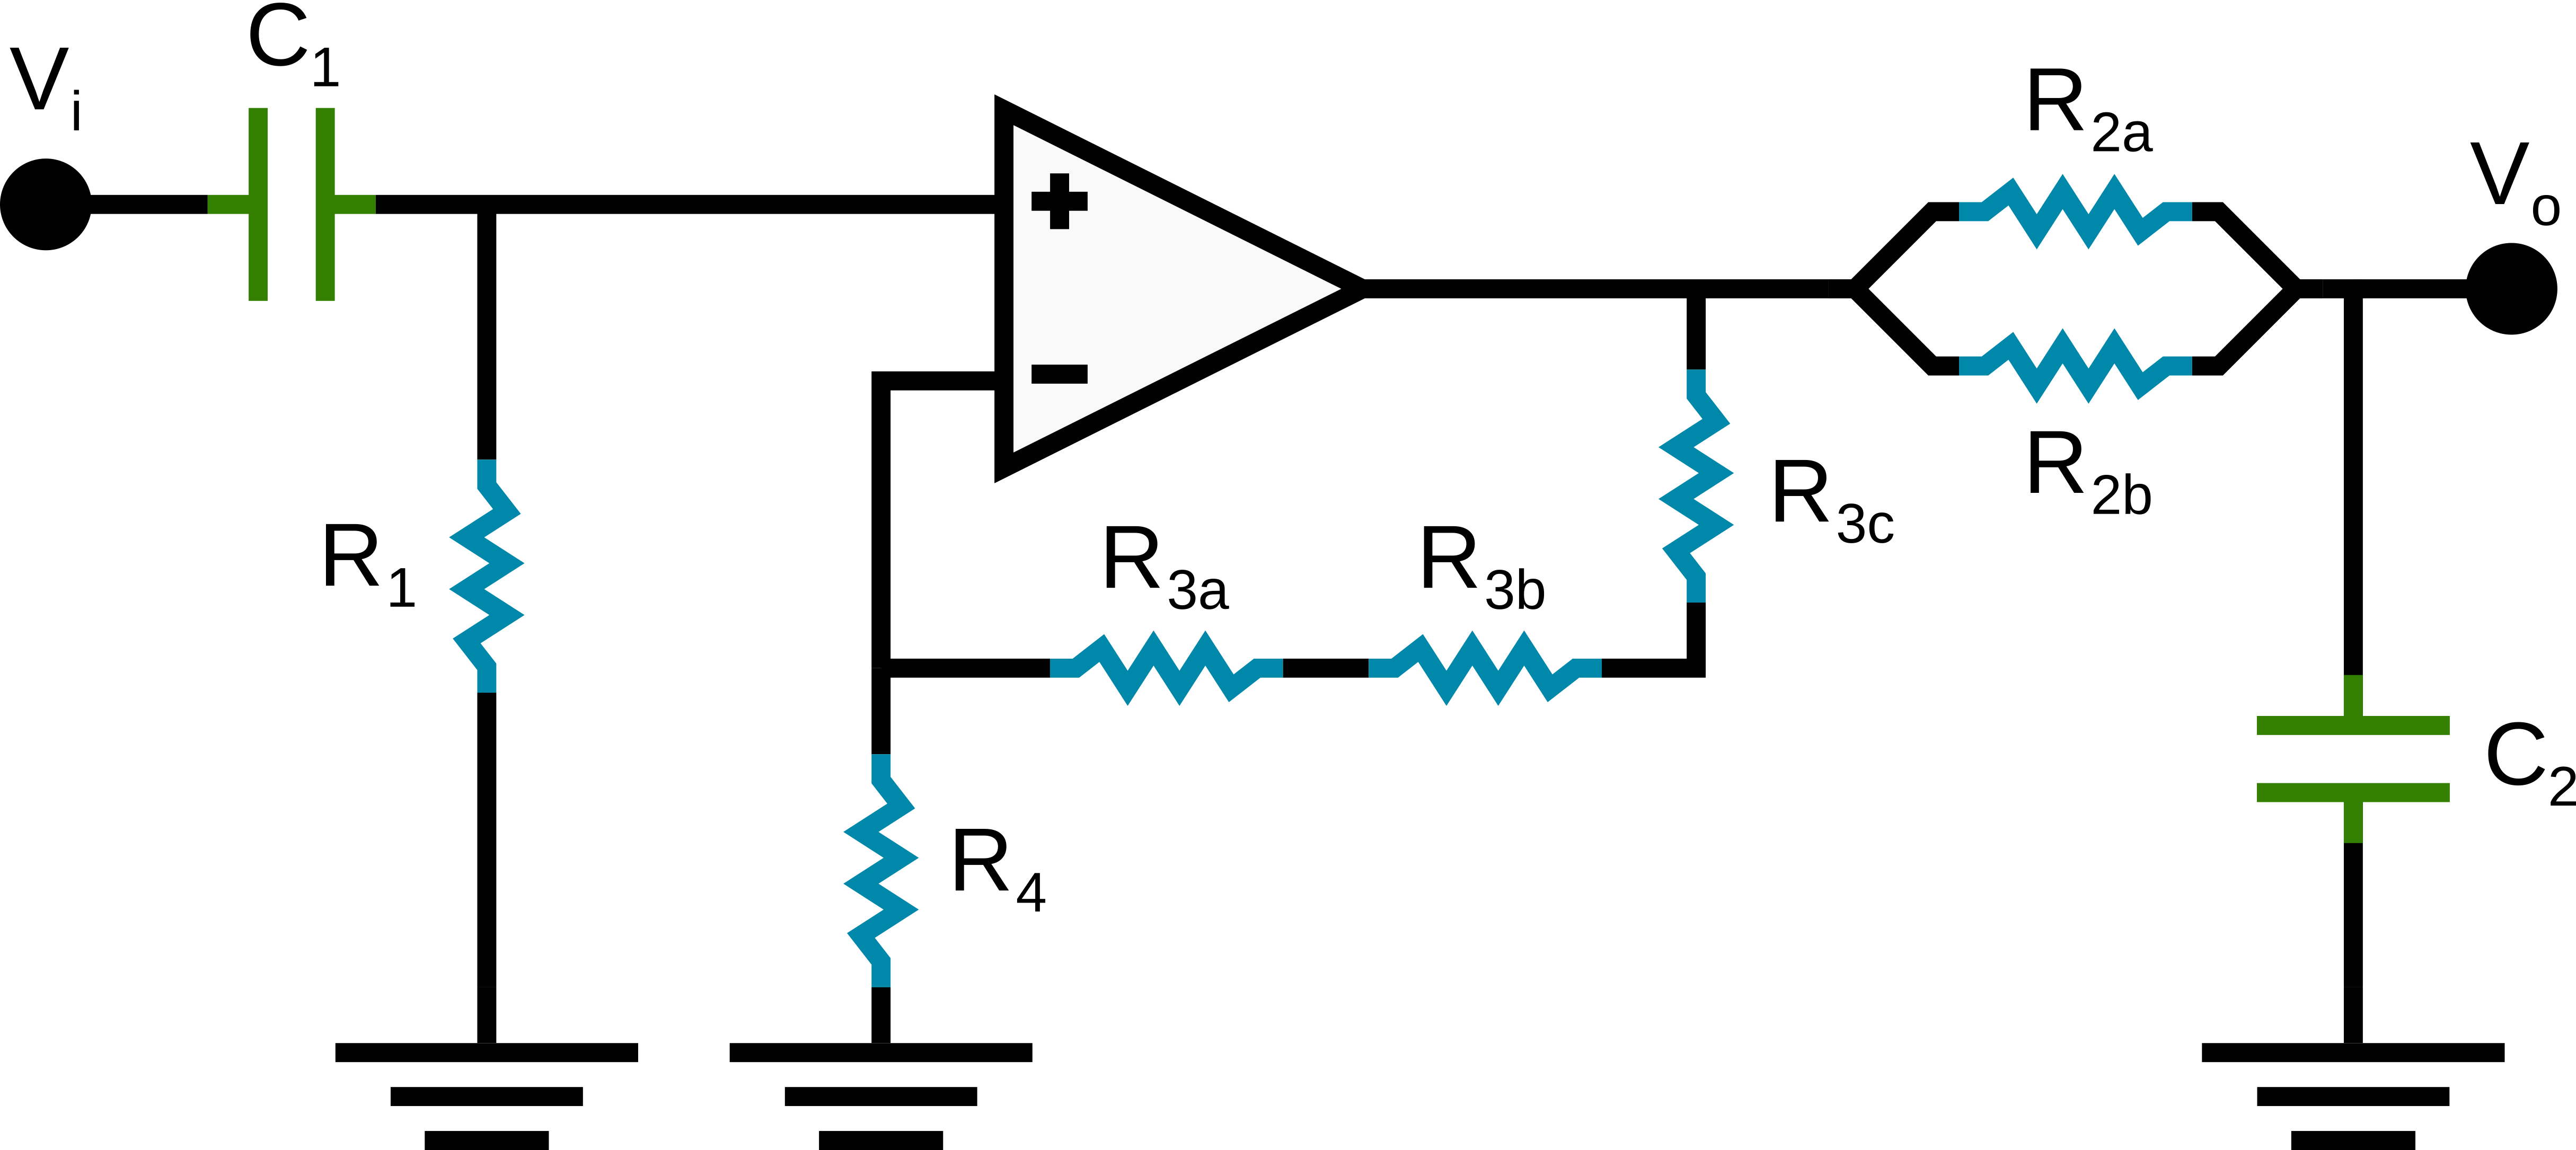
\includegraphics[width=\linewidth]{circuit.png}
  \vspace{1cm}
  \caption{Amplifier circuit}
  \label{fig:circuit}
  \hfill
\end{figure}


\FloatBarrier
